% Importado desde: 2026-03-28_Isotropia_y_Simetrias_en_QW_Honeycomb.tex
\chapter{Derivacion Pedagogica: --- isotropia y estructura de simetrias --- en una quantum walk concreta tipo honeycomb/triangular}
\label{ch:isotropia-qw-honeycomb}

\section{Objetivo}
Despues de comparar tiempo continuo con tiempo discreto, el paso natural era dejar de hablar en abstracto y tomar una construccion concreta. Eso es lo que haremos ahora con una \textit{quantum walk} orientada por las tres direcciones naturales de la geometria tipo honeycomb/triangular.

Las dos preguntas centrales del capitulo son:
\begin{displayquote}
\textbf{por que una dinamica definida sobre una red que no es isotropa de manera continua puede, sin embargo, producir una teoria efectiva isotropa en baja energia?}
\end{displayquote}
\begin{displayquote}
\textbf{que simetrias son verdaderamente microscopicas en la caminata, y cuales aparecen solo en el limite efectivo tipo Dirac?}
\end{displayquote}

Estas preguntas importan mucho para el proyecto porque una lectura de proto-espacio-tiempo no puede apoyarse solo en \enquote{parecidos} con Dirac. Necesita entender exactamente:
\begin{enumerate}[label=\arabic*.]
    \item de donde sale la isotropia;
    \item que tan robusta es;
    \item y bajo que grupo de simetrias debe leerse.
\end{enumerate}

\section{La caminata concreta}
\subsection{Tres direcciones espaciales}
Tomamos las tres direcciones de primeros vecinos:
\begin{equation}
\vdelta_1 = a(0,-1),
\qquad
\vdelta_2 = a\left(\frac{\sqrt{3}}{2},\frac{1}{2}\right),
\qquad
\vdelta_3 = a\left(-\frac{\sqrt{3}}{2},\frac{1}{2}\right),
\label{c05:eq:deltas}
\end{equation}
con la propiedad geometrica clave
\begin{equation}
\vdelta_1+\vdelta_2+\vdelta_3 = 0.
\label{c05:eq:sumzero}
\end{equation}

Si definimos \(\hat{\vdelta}_i=\vdelta_i/a\), entonces la caminata usa estas tres direcciones como base elemental de propagacion.

\begin{figure}[h!]
\centering
\begin{tikzpicture}[scale=1.5,>=Latex]
  \coordinate (O) at (0,0);
  \coordinate (D1) at (0,-1);
  \coordinate (D2) at (0.866,0.5);
  \coordinate (D3) at (-0.866,0.5);
  \fill[black] (O) circle (1.8pt);
  \draw[->,very thick,red!70!black] (O) -- (D1) node[midway,right] {\small \(\vdelta_1\)};
  \draw[->,very thick,green!60!black] (O) -- (D2) node[midway,above right] {\small \(\vdelta_2\)};
  \draw[->,very thick,blue!70!black] (O) -- (D3) node[midway,above left] {\small \(\vdelta_3\)};
  \node[below] at (0,-1.25) {\small tres direcciones de propagacion};
  \node[above] at (0,1.1) {\small \(\vdelta_1+\vdelta_2+\vdelta_3=0\)};
\end{tikzpicture}
\caption{La geometria espacial minima de la caminata. Microscópicamente solo hay tres direcciones privilegiadas.}
\end{figure}

\subsection{Espacio interno}
Introducimos un espacio interno de dos componentes y asociamos a cada direccion una matriz interna
\begin{equation}
\tau_i = \hat{\delta}_i^x \sigma_x + \hat{\delta}_i^y \sigma_y.
\label{c05:eq:taui}
\end{equation}

Explícitamente:
\begin{equation}
\tau_1 = -\sigma_y,
\qquad
\tau_2 = \frac{\sqrt{3}}{2}\sigma_x + \frac{1}{2}\sigma_y,
\qquad
\tau_3 = -\frac{\sqrt{3}}{2}\sigma_x + \frac{1}{2}\sigma_y.
\label{c05:eq:taus}
\end{equation}

Este es el punto fino del modelo: la estructura interna copia la geometria angular de las direcciones de propagacion.

\subsection{Paso elemental}
Tomamos un paso unitario de la forma
\begin{equation}
U = S_3 S_2 S_1 C_m,
\label{c05:eq:U}
\end{equation}
donde
\begin{equation}
S_i = \ee^{-\,\ii \varepsilon v \tau_i p_i},
\qquad
p_i = \hat{\vdelta}_i\cdot \vp,
\qquad
\vp = -\ii \nabla,
\label{c05:eq:Si}
\end{equation}
y
\begin{equation}
C_m = \ee^{-\,\ii \varepsilon m \sigma_z}.
\label{c05:eq:Cm}
\end{equation}

La interpretacion es transparente:
\begin{enumerate}[label=\arabic*.]
    \item cada \(S_i\) empuja la dinamica en una de las tres direcciones naturales;
    \item \(C_m\) introduce el termino de masa efectivo.
\end{enumerate}

\section{Primer analisis: el Hamiltoniano efectivo}
Para \(\varepsilon\ll 1\) expandimos:
\begin{equation}
S_i \simeq \bbI - \ii \varepsilon v \tau_i p_i,
\qquad
C_m \simeq \bbI - \ii \varepsilon m \sigma_z.
\end{equation}

Entonces:
\begin{equation}
U \simeq \bbI - \ii \varepsilon
\left(
v\sum_{i=1}^3 \tau_i p_i + m\sigma_z
\right).
\end{equation}

Por comparacion con \(U\simeq \bbI - \ii\varepsilon H_{\text{eff}}\), obtenemos
\begin{equation}
H_{\text{eff}} =
v\sum_{i=1}^3 \tau_i p_i + m\sigma_z.
\label{c05:eq:Heffraw}
\end{equation}

\subsection{La cuenta central}
Ahora hacemos la cuenta que realmente decide la isotropia.

Usamos
\begin{equation}
p_1 = -p_y,
\qquad
p_2 = \frac{\sqrt{3}}{2}p_x + \frac{1}{2}p_y,
\qquad
p_3 = -\frac{\sqrt{3}}{2}p_x + \frac{1}{2}p_y.
\label{c05:eq:pi}
\end{equation}

Entonces:
\begin{equation}
\tau_1 p_1 = (-\sigma_y)(-p_y)=\sigma_y p_y.
\end{equation}

Por otro lado,
\begin{align}
\tau_2 p_2
&=
\left(
\frac{\sqrt{3}}{2}\sigma_x + \frac{1}{2}\sigma_y
\right)
\left(
\frac{\sqrt{3}}{2}p_x + \frac{1}{2}p_y
\right)
\notag\\
&=
\frac{3}{4}\sigma_x p_x
+ \frac{\sqrt{3}}{4}\sigma_x p_y
+ \frac{\sqrt{3}}{4}\sigma_y p_x
+ \frac{1}{4}\sigma_y p_y,
\end{align}
y
\begin{align}
\tau_3 p_3
&=
\left(
-\frac{\sqrt{3}}{2}\sigma_x + \frac{1}{2}\sigma_y
\right)
\left(
-\frac{\sqrt{3}}{2}p_x + \frac{1}{2}p_y
\right)
\notag\\
&=
\frac{3}{4}\sigma_x p_x
- \frac{\sqrt{3}}{4}\sigma_x p_y
- \frac{\sqrt{3}}{4}\sigma_y p_x
+ \frac{1}{4}\sigma_y p_y.
\end{align}

Al sumar:
\begin{equation}
\sum_{i=1}^3 \tau_i p_i
=
\frac{3}{2}\sigma_x p_x + \frac{3}{2}\sigma_y p_y.
\label{c05:eq:keysum}
\end{equation}

Por tanto,
\begin{equation}
H_{\text{eff}}
=
\frac{3v}{2}\left(\sigma_x p_x + \sigma_y p_y\right)
+ m\sigma_z.
\label{c05:eq:Dirac2p1}
\end{equation}

\section{Por que esto significa isotropia efectiva}
El resultado \eqref{c05:eq:Dirac2p1} es crucial. Aunque la microdinamica distinguia tres direcciones concretas, el Hamiltoniano efectivo solo depende de la combinacion
\begin{equation}
\sigma_x p_x + \sigma_y p_y,
\end{equation}
que es la forma canonica de Dirac en \(2+1\).

\subsection{Espectro}
El espectro viene dado por
\begin{equation}
E(\vp)=\pm\sqrt{m^2+\left(\frac{3v}{2}\right)^2(p_x^2+p_y^2)}.
\label{c05:eq:disp}
\end{equation}

Luego las curvas de energia constante satisfacen
\begin{equation}
p_x^2+p_y^2 = \text{constante},
\end{equation}
es decir: son circunferencias en el espacio de momentos.

\subsection{Lectura fisica}
Aqui esta la leccion fuerte:
\begin{displayquote}
\textbf{la red no es isotropa de manera continua, pero la suma coherente de las tres direcciones recupera una teoria infrarroja isotropa.}
\end{displayquote}

Esta es exactamente la clase de fenomeno que necesitamos en el proyecto: una simetria efectiva mas grande que la simetria microscopica.

\begin{figure}[h!]
\centering
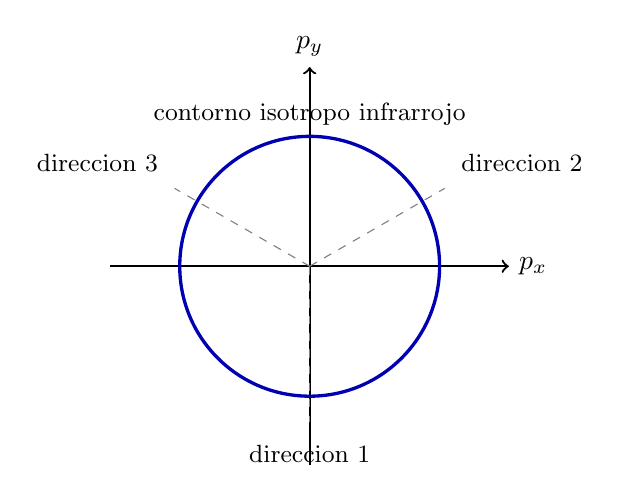
\begin{tikzpicture}[scale=1.1]
  \draw[->,thick] (-2.3,0) -- (2.3,0) node[right] {\(p_x\)};
  \draw[->,thick] (0,-2.3) -- (0,2.3) node[above] {\(p_y\)};
  \draw[very thick,blue!70!black] (0,0) circle (1.5);
  \draw[gray,dashed] (0,0) -- (0,-1.8);
  \draw[gray,dashed] (0,0) -- (1.56,0.9);
  \draw[gray,dashed] (0,0) -- (-1.56,0.9);
  \node[below] at (0,-1.95) {\small direccion 1};
  \node[above right] at (1.64,0.98) {\small direccion 2};
  \node[above left] at (-1.64,0.98) {\small direccion 3};
  \node at (0,1.75) {\small contorno isotropo infrarrojo};
\end{tikzpicture}
\caption{La microgeometria tiene tres direcciones privilegiadas, pero la dispersion efectiva ya no recuerda esa anisotropia a primer orden.}
\end{figure}

\section{Segundo analisis: las simetrias microscopicas}
Ahora toca distinguir con cuidado que simetrias tiene realmente la caminata antes de pasar al continuo.

\subsection{Traslaciones discretas}
La primera simetria es la invariancia bajo traslaciones de la red. La regla local es la misma en cada celda, por lo que el modelo es homogéneo.

\subsection{Rotacion discreta de \(2\pi/3\)}
La geometria admite una rotacion espacial de \(120^\circ\) que permuta
\begin{equation}
\vdelta_1 \to \vdelta_2 \to \vdelta_3 \to \vdelta_1.
\end{equation}

Pero como la estructura interna esta alineada con esas direcciones, la rotacion espacial debe acompa\~narse de una rotacion en el espacio espinorial.

\subsection{Rotacion interna asociada}
Definimos
\begin{equation}
V(\phi)=\ee^{-\,\ii \frac{\phi}{2}\sigma_z}.
\label{c05:eq:Vphi}
\end{equation}

Entonces:
\begin{align}
V(\phi)\sigma_x V(\phi)^\dagger &= \cos\phi\,\sigma_x + \sin\phi\,\sigma_y,\\
V(\phi)\sigma_y V(\phi)^\dagger &= -\sin\phi\,\sigma_x + \cos\phi\,\sigma_y.
\end{align}

Para \(\phi=2\pi/3\), esto rota exactamente los vectores internos \(\tau_i\) del mismo modo que la rotacion espacial permuta las direcciones \(\vdelta_i\). Por tanto, el paso \(U\) es invariante bajo una \textbf{simetria combinada}:
\begin{equation}
\text{rotacion espacial de } 2\pi/3
\quad+\quad
\text{rotacion interna } V(2\pi/3).
\label{c05:eq:combined}
\end{equation}

\begin{figure}[h!]
\centering
\begin{tikzpicture}[scale=1.2,>=Latex]
  \node[draw,rounded corners,fill=blue!8,minimum width=3.3cm,minimum height=0.9cm,align=center] (a) at (0,0) {rotacion espacial\\\(\vdelta_1\to \vdelta_2\to \vdelta_3\)};
  \node[draw,rounded corners,fill=green!8,minimum width=3.3cm,minimum height=0.9cm,align=center] (b) at (5.1,0) {rotacion interna\\\(\tau_1\to \tau_2\to \tau_3\)};
  \node[draw,rounded corners,fill=orange!10,minimum width=4cm,minimum height=0.95cm,align=center] (c) at (10.7,0) {simetria combinada\\del paso \(U\)};
  \draw[->,thick] (a) -- (b);
  \draw[->,thick] (b) -- (c);
\end{tikzpicture}
\caption{La simetria relevante no es una rotacion espacial sola, sino una rotacion combinada espacio + espacio interno.}
\end{figure}

\subsection{Masa}
El termino \(m\sigma_z\) es invariante bajo \(V(\phi)\), porque \(\sigma_z\) conmuta con esa rotacion. Luego la masa no rompe la simetria discreta de \(120^\circ\).

\section{Tercer analisis: las simetrias efectivas}
Una vez linealizado el modelo, la estructura de simetrias se reorganiza.

\subsection{Rotaciones continuas emergentes}
El Hamiltoniano efectivo
\begin{equation}
H_{\text{eff}} =
v_\ast(\sigma_x p_x + \sigma_y p_y)+m\sigma_z,
\qquad
v_\ast=\frac{3v}{2},
\end{equation}
es invariante bajo rotaciones continuas en el plano si las acompa\~namos con la rotacion espinorial adecuada.

\subsection{Generador}
El generador efectivo es
\begin{equation}
J_z = L_z + \frac{1}{2}\sigma_z.
\label{c05:eq:Jz}
\end{equation}

Esto significa que la simetria continua \(SO(2)\) no estaba presente microscópicamente: emerge solo en el infrarrojo, cuando el sistema ya no resuelve la estructura angular fina de la red.

\subsection{Leccion}
La relacion entre micro y macro puede resumirse asi:
\begin{equation}
C_3 \quad \longrightarrow \quad SO(2)_{\text{efectivo}}.
\end{equation}

No es una igualdad exacta, sino una emergencia de simetria al pasar a longitudes de onda grandes.

\section{Cuarto analisis: que no debemos sobreinterpretar}
Este punto es delicado y conviene dejarlo muy claro.

\subsection{No hay isotropia exacta a toda escala}
La isotropia que obtuvimos vale en la expansion de baja energia. A escalas de red, la caminata sigue recordando las tres direcciones privilegiadas.

\subsection{No hay todavia Lorentz completa}
El modelo reconstruye muy bien la parte cinetica de Dirac en \(2+1\), pero eso no significa que ya tengamos la simetria de Lorentz completa como simetria microscopica.

\subsection{No hay aun tiempo emergente universal}
Aunque la caminata ya discreta el tiempo, todavia falta demostrar que el tiempo continuo efectivo reconstruido por el limite infrarrojo sea universal y suficientemente robusto frente a deformaciones del paso.

\section{Quinto analisis: simetrias discretas delicadas}
Aqui conviene distinguir entre el modelo reducido de un solo cono y una teoria microscopica completa.

\subsection{Reversion temporal}
En una teoria efectiva de un solo espinor de Dirac en \(2+1\), el analisis de inversion temporal es sutil. En particular, el termino de masa \(m\sigma_z\) no debe interpretarse ingenuamente como si respetara todas las simetrias que uno esperaria de una teoria con dos valles.

\subsection{Leccion de metodo}
Si queremos hablar en serio de reversion temporal, inversion o estructuras tipo grafeno completas, hay que controlar tambien:
\begin{enumerate}[label=\arabic*.]
    \item duplicacion de conos;
    \item sectores de valle;
    \item accion precisa de las simetrias antiunitarias en el espacio completo de estados.
\end{enumerate}

Para este capitulo no necesitamos entrar tan lejos. Lo importante es no confundir:
\begin{enumerate}[label=\arabic*.]
    \item la simetria discreta real de la caminata;
    \item con simetrias efectivas de un bloque reducido;
    \item o con simetrias aun mas grandes del continuo relativista.
\end{enumerate}

\section{Que nos dice esto sobre proto-espacio-tiempo}
Ahora ya podemos volver a la pregunta grande del proyecto.

\subsection{Lo positivo}
Este modelo muestra de forma muy convincente que:
\begin{enumerate}[label=\arabic*.]
    \item una dinamica discreta local puede producir una teoria isotropa en el infrarrojo;
    \item la isotropia efectiva puede emerger de una simetria microscopica mucho mas pobre;
    \item la estructura interna del caminante no es un adorno: es la pieza que permite recombinar las direcciones y formar un operador de Dirac.
\end{enumerate}

\subsection{Lo que aun falta}
Para acercarnos mas a una lectura de proto-espacio-tiempo todavia faltan al menos tres cosas:
\begin{enumerate}[label=\arabic*.]
    \item controlar mejor la extension a \(3D\);
    \item entender como emergen simetrias mas cercanas a Lorentz;
    \item verificar la robustez de la isotropia frente a deformaciones del paso unitario.
\end{enumerate}

\begin{figure}[h!]
\centering
\begin{tikzpicture}[
    box/.style={draw, rounded corners, thick, align=center, minimum width=4cm, minimum height=1.05cm},
    arr/.style={-{Latex[length=3mm]}, thick}
]
\node[box, fill=blue!7] (a) at (0,0) {microgeometria\\con \(3\) direcciones};
\node[box, fill=green!7] (b) at (4.8,0) {estructura interna\\alineada};
\node[box, fill=yellow!12] (c) at (9.6,0) {Dirac isotropo\\en el infrarrojo};
\node[box, fill=red!7] (d) at (14.4,0) {candidato mas serio\\de proto-geometria};
\draw[arr] (a) -- (b);
\draw[arr] (b) -- (c);
\draw[arr] (c) -- (d);
\end{tikzpicture}
\caption{La logica del capitulo: la isotropia efectiva no cae del cielo, sino de una combinacion precisa entre geometria y espacio interno.}
\end{figure}

\section{Tabla de lectura}
\begin{center}
\begin{tabular}{p{4.1cm} p{4.8cm} p{5.3cm}}
\toprule
Nivel & Simetria dominante & Comentario \\
\midrule
Microscopico & traslaciones discretas + \(C_3\) combinado & la red no es continuamente isotropa \\
Paso unitario & regla local \(U=S_3S_2S_1C_m\) & la estructura interna acompa\~na la geometria \\
Infrarrojo & isotropia efectiva \(SO(2)\) & emerge tras linealizar \\
Interpretativo & proto-geometria posible & solo si la isotropia es robusta y extendible \\
\bottomrule
\end{tabular}
\end{center}

\section{Mapa del siguiente paso}
El analisis de este capitulo deja bastante claro cual es el siguiente paso natural del programa:
\begin{displayquote}
\textbf{estudiar que condiciones debe satisfacer una caminata o QCA en \(3D\) para que una isotropia efectiva análoga sobreviva y pueda organizarse en torno a una estructura tipo Weyl o Dirac.}
\end{displayquote}

Ese paso ya no sera solo una repeticion del caso \(2D\). Habra que decidir:
\begin{enumerate}[label=\arabic*.]
    \item cuantas direcciones espaciales elementales hacen falta;
    \item que espacio interno minimo es necesario;
    \item y bajo que simetria discreta puede emerger una teoria efectivamente isotropa en tres dimensiones.
\end{enumerate}

\section{Resumen final}
La conclusion mas importante del capitulo es que la isotropia efectiva no contradice la discrecion microscopica. Una caminata definida sobre una geometria con solo tres direcciones privilegiadas puede, gracias a una eleccion muy precisa de su estructura interna, recombinar esas direcciones en un Hamiltoniano de Dirac isotropo a baja energia.

Tambien queda clara la jerarquia de simetrias. Microscópicamente la caminata solo posee traslaciones discretas y una simetria rotacional discreta combinada con el espacio interno. En el infrarrojo, en cambio, emerge una simetria rotacional continua mucho mas rica. Justamente esa diferencia entre simetria microscopica pobre y simetria efectiva grande es una de las se\~nales mas prometedoras de todo el proyecto.
